% -*- mode: fundamental -*-

% ****************************************************************

\chapter{RISC-V: the Fife pipelined CPU code}

\markboth{Ch \arabic{chapter}: Fife code}{\copyrightnotice}

\setcounter{page}{1}
% \renewcommand{\thepage}{\arabic{page}}
\renewcommand{\thepage}{\arabic{chapter}-\arabic{page}}

\label{ch_Fife_code}

% ****************************************************************

\section{Introduction}

In this chapter we study BSV code to implement the principles that
were discussed in Chapter~\ref{ch_Fife_Principles}.
We repeat Figure~\ref{Fig_Instr_Exec_w_FIFOs} here, for reference.
\begin{figure}[htbp]
  \centerline{\includegraphics[width=6in,angle=0]{Figures/Fig_Instr_Exec_w_FIFOs}}
  \caption{\label{Fig_Instr_Exec_w_FIFOs_2}Pipelined interpretation of RISC-V instructions (Fig.~\ref{Fig_Instr_Exec} with some annotations)}
\end{figure}

% ****************************************************************

\section{The Fife top-level CPU module}

\label{Sec_Fife_CPU_module}

The code for the top-level Fife CPU module is actually simpler than
the code for the Drum CPU module, because it simply instantiates
sub-modules for each stage and connects them:

\input{Code_Extracts/Fife_mkCPU.tex}

This is practically a direct textual description of
Figure~\ref{Fig_Instr_Exec_w_FIFOs_2}.  The STATE section first
instantiates the pipeline stages shown in the figure.  There is no
explicit module corresponding to Execute Memory Ops---the DMem request
is sent out directly from \verb|stage_RR_RW| and the DMem response is
collected directly by \verb|stage_Retire|.

The STATE section then instantiates the ``forward-flow'' connections
between modules (left to right in the figure), using the
\verb|mkConnection| module to connect a \verb|FIFOF_O| interface
(producer) to a \verb|FIFOF_I| interface (consumer), which was
discussed in Section~\ref{Sec_connecting_FIFOs}.  These module
connections are in the STATE section because, as discussed in
Section~\ref{Sec_connecting_FIFOs} \verb|mkConnection| is just a
module instantiation.

The next few lines instantiate the ``backward-flow'' connections.

In the INTERFACE section, after the \verb|init| method, the next two
lines are the flows of IMem requests from the Fetch stage to memory
and IMem responses from memory to the Decode stage.  These just lift
interfaces from \verb|stage_F| and \verb|stage_D| to the CPU
interface, as is.

The next three lines are for \emph{speculative} DMem access, which we
discussed in Section~\ref{Sec_Store_Buffers}: the flow of DMem
requests from \verb|stage_RR| to memory, the flow of DMem responses
from memory to \verb|stage_Retire|, and the flow of ``commit/discard''
messages from \verb|stage_Retire| to the store-buffer to discharge
STOREs that are waiting in the store-buffer.

The last two lines are for \emph{non-speculative} DMem access, which
we discussed in Section~\ref{Sec_DMem_MMIO}.

Note that the module interface \verb|CPU_IFC| is exactly the same as
in Drum (although Drum has no need for, and does not use the
\verb|DMem_S| speculative interfaces).  Thus, in a system context, we
can directly substitute Drum for Fife and vice versa.  Generalizing
this idea, we can develop other CPUs and substitute them, as well.

We next go through the code for the individual stage modules.

% ****************************************************************

\section{The Fetch stage}

\label{Sec_Fife_Fetch_stage}

The Fetch stage module interface is shown below.  Apart from the
\verb|init| method, the remaining sub-interfaces correspond to the
FIFO-labeled arrows in Figure~\ref{Fig_Instr_Exec_w_FIFOs_2}: the
outgoing \verb|FIFOF_O| interfaces to memory (IMem) and the Decode
stage, and the incoming \verb|FIFOF_I| for redirections from the
Retire stage.

\input{Code_Extracts/Fife_Fetch_IFC.tex}

The Fetch stage module code is shown below.

\input{Code_Extracts/Fife_mkFetch.tex}

The STATE section instantiates various registers and FIFOs.  Next, the
BEHAVIOR section contains two \emph{rules} (Chapter~\ref{ch_Rules}).
In rule \verb|rl_Fetch_req|, the explicit condition is the expression:

\hm\small \verb|(rg_running && (! f_F_from_Retire.notEmpty))|

Rule \verb|rl_Fetch_req|'s implicit condition comes from the methods
that it invokes, \verb|f_Fetch_to_Decode.enq ()| and
\verb|f_Fetch_to_IMem.enq ()|.  The rule will fire only when the
explicit condition is true, and when both FIFOs are enabled to enqueue
(have space).  When it fires, it performs the composite action that
comprises all the actions in the rule body:


\begin{itemize}

 \item enqueue the value of \verb|y.to_D| into FIFO \verb|f_Fetch_to_Decode|;

 \item enqueuethe value of \verb|y.mem_req| into FIFO \verb|f_Fetch_to_IMem|;

 \item write the predicted PC value \verb|pred_pc| into register \verb|rg_pc|, and

 \item write the value of \verb|rg_inum+1| into the register \verb|rg_inum|.

\end{itemize}

The right-hand side expressions (\verb|rg_pc+4|, \verb|fn_Fetch(...)| and
\verb|rg_inum+1|) are all combinational circuits, and ``\verb|y|'' is
not a register, just a name for the wires carrying the output value of
\verb|fn_Fetch()|.

% ----------------

\vspace{1ex}

NOTE:
\fbox{\small
\begin{minipage}{5in}

The function {\tt fn\_Fetch()} is exactly the same as the one used in
the Fetch step of Drum (was described in Section~\ref{Sec_fn_Fetch}).

\vspace{1ex}

The types of the messages passed to the Decode stage ({\tt y.to\_D} of
type {\tt F\_to\_D}) and to memory ({\tt y.mem\_req} of type {\tt
Mem\_Req}) are the same as in Drum.

\end{minipage}}

\vspace{1ex}

% ----------------

All these actions are semantically \emph{instantaneous} and
\emph{simultaneous}.  Note that when the rule's implicit and explicit
conditions are true, all the actions are peformed; if false, none of
them are performed, {\ie} the rule is ``atomic''.

In summary, rule \verb|rl_Fetch_req| computes an IMem memory request
from the PC and sends it to memory; it sends auxiliary information to
the Decode stage; and it updates the PC and inum in preparation for
the next Fetch (the next firing of the rule)..

The second rule in the module is \verb|rl_Fetch_from_Retire|. It
receives, in \verb|x|, a redirection message from the Retire stage,
and updates the PC and epoch accordingly.  This rule has no explicit
conditions; its single implicit condition comes from
\verb|f_Fetch_from_Retire|'s implicit condition that we cannot pop a
value from the FIFO until it is non-empty, {\ie}, this rule only fires
when a redirection message is available.  When it fires, it performs
three actions atomically/instantaneously/simultaneously:
 
\begin{itemize}

 \item It dequeues \verb|x| from the FIFO \verb|f_F_from_Retire| (the
       dequeue action is inside the \verb|pop_o| function),
 \item It updates \verb|rg_pc| with the new PC in the redirection message,
 \item It updates \verb|rg_epoch| with the new epoch in the redirection message.

\end{itemize}

Note, \verb|rl_Fetch_from_Retire| updates two registers \verb|rg_pc|
and \verb|rg_epoch| and, \emph{concurrently}, \verb|rl_Fetch| reads
both those registers.  Because rule actions are atomic, we are
guaranteed that \verb|rl_Fetch| will not see inconsitent values in
those two registers, where one has been updated but the other has not
yet been updated.

Finally, the INTERFACE section of the module is simple.  After the
\verb|init| method, we simply lift the FIFO interfaces to the
\verb|mkFetch| module interface.

% ================================================================

\subsection{Prioritizing rule {\tt rl\_Fetch\_from\_Retire} over {\tt rl\_Fetch\_req}}

\index{Rules!prioritizing explicitly}

What would happen if we omit the condition
``\verb|(!f_Fetch_from_Retire.notEmpty)|'' in \verb|rl_Fetch_req|?  It
would not affect the correctness of this module at all.  If we omit
the condition, then both rules could be enabled simultaneously, and it
is non-deterministic which one will fire first.  Actually, the
hardware is deterministic because the \emph{bsc} compiler will make a
prioritization choice, but its choice is unspecified, and so
semantically it is non-deterministic ({\eg} a new release of the
compiler, or a later change in other code in the module may prioritize
differently).  But, for correctness, the choice \emph{does not
matter}.  Because of the atomicity of rules, the rules will never
\emph{interleave} their behavior---either one goes before the other,
or vice versa.  We can quickly reason that, in either case, we get
functionally correct behavior.

The only difference will be in performance: if both rules are enabled,
then, by definition, \verb|rl_Fetch| is fetching ``wrong-path''
instructions due to an earlier misprediction (which is why we have a
redirection).  We know that wrong-path instructions will be discarded
and have no effect.  So if \verb|rl_Fetch| is prioritized, it will
fetch one more wrong-path instruction, with no impact on correctness.

By adding the ``\verb|(!f_Fetch_from_Retire.notEmpty)|'' condition to
\verb|rl_Fetch|, we are explicitly prioritizing
\verb|rl_Fetch_from_Retire| when both are enabled, thus avoiding
\verb|rl_Fetch_req| performing a wasted wrong-path fetch.

% ****************************************************************

\section{The Decode stage}

\label{Sec_Fife_Decode_stage}

The Decode stage module interface is shown below.  Apart from the
\verb|init| method, the remaining sub-interfaces correspond to the
FIFO-labeled arrows in Figure~\ref{Fig_Instr_Exec_w_FIFOs_2}: the
incoming \verb|FIFOF_I| interfaces from the Fetch stage and memory
(IMem), and the outgoing \verb|FIFOF_O| interface to the Register-Read
stage.

\input{Code_Extracts/Fife_Decode_IFC.tex}

The Decode stage module code is shown below.

\input{Code_Extracts/Fife_mkDecode.tex}

The STATE section instantiates FIFOs for incoming and outgoing flows.

The BEHAVIOR section has the single rule \verb|rl_Decode|, whose
implicit conditions will make it wait for both incoming FIFOs
\verb|f_Fetch_to_Decode| and \verb|f_IMem_to_Decode| to be non-empty,
and for its outgoing FIFO \verb|f_Decode_to_RR| to have space.  When
the rule fires, it:

\begin{tightlist}
 \item pops \verb|x| and \verb|rsp_Mem| from the two FIFOs, respectively;

 \item applies function \verb|fn_Decode()| to those values (this is
       the \emph{same} \verb|fn_Decode()| that was used in the Decode
       step of Drum, and described in Section~\ref{Sec_fn_Decode}),
       and

 \item sends the result on to the Register-Read stage.
\end{tightlist}

The INTERFACE section is again straightforward, just lifting the FIFO
interfaces to this module's interface.

% ================================================================

\subsection{Balancing concurrent paths in a pipeline}

\label{Sec_Balancing}

\index{RISC-V!Balancing concurrent paths in a pipeline}

In Figure~\ref{Fig_Instr_Exec_w_FIFOs_2} we see that there are two
concurrent FIFO-like paths from Fetch to Decode: one direct, and the
other via memory (IMem).  Fetch produces two outputs together, one for
each path.  The paths re-converge at Decode, where Fetch's first
output ``meets'' the corresponding response from memory.

\index{RISC-V!In-flight memory transactions}
\index{RISC-V!Memory!pipelined}
\index{RISC-V!Memory!latency}

The path via IMem is also FIFO-like because good memory systems are
themselves pipelined; it is possible for Fetch to issue several
consecutive memory requests before the first response arrives at
Decode.  We say that multiple IMem transactions may be ``in flight''.
Also, in Section~\ref{Sec_mem_latency} we discussed how memory latency
can be variable and unpredictable, so the number of transactions in
flight may vary.

If we wish to allow up to $n$ IMem transactions in flight, then the
direct Fetch-to-Decode path must be capable of buffering up to $n$
\verb|Fetch_to_Decode| items.  If not, rule \verb|rl_Fetch| in Fetch
will get stuck: its \verb|f_Fetch_to_Decode| FIFO will be full, and so
the ``\verb|enq|'' method's implicit condition will become false,
preventing the rule from firing.

This is the reason, in Decode, the incoming \verb|f_Fetch_to_Decode|
FIFO is instantiated with \verb|mkSizedFIFOF(4)|, which is a FIFO with
the capacity to hold four items\footnote{We could also have,
equivalently, instantiated the {\tt f\_Fetch\_to\_Decode} FIFO in
Fetch with {\tt mkSizedFIFO}, or split the buffering capacity between
the two stages.}  We also use the term ``balancing'' for this---the
number of items that can be ``in flight'' in the two paths should be
matched.

Why did we choose the number 4?  Why not something smaller, or larger?
Greater capacity requires more hardware resources, which argues for a
smaller number, but a smaller number may affect performance where
Fetch has to wait only because of limited capacity.  We would like to
choose the smallest number that covers the number of IMem transactions
that may be in flight (memory latency, or depth of IMem pipeline).
But that number varies with memory system design and, even for a
particular design, it varies over time---it depends on the particular
RISC-V program running, the memory system's caches, hits and misses,
cache interactions, cache miss latencies, and so on\footnote{With
virtual memory, it will also depend on TLB misses and the latency of
page table walks.}  Thus, there is no obvious ``optimal'' choice for
\verb|mkSizedFIFOF| capacity; we must ``tune'' the number by running
the CPU on desired applications, with different FIFO capacities,
observe the effect on performance and resources, and pick an
``acceptable'' capacity.

% ****************************************************************

\section{The Register-Read and Dispatch (and Register-Write) stage}

\label{Sec_Fife_RR_RW_stage}

The Register-Read and Dispatch module contains (instantiates) the GPRs
register file (Section~\ref{Sec_RISCV_regfile}) and the scoreboard to
manage read-write hazards (Section~\ref{Sec_Scoreboards}).  In the
forward flow,

\begin{itemize}

  \item it stalls (waits) if the instruction has rs1, rs2 or rd, and
        these are busy according to the scoreboard;

  \item it reads rs1 and rs2 registers for the current instruction;

  \item it sets the scoreboard for the current instruction's rd to 1,
        marking it ``busy'' (if the instruction has an rd);

  \item it uses information from the Decode stage to dispatch to the
        four Execute pipes.  We always (for every instruction) send an
        execution tag and additional information on the direct path to
        Retire.  Depending on the instruction, it may also send
        information into one of the other Execute pipes:

  \begin{tightlist}
    \item Execute Control
    \item Execute Integer
    \item memory (a DMem request)
  \end{tightlist}

\end{itemize}

This stage also participates in a backward flow, because the GPRs
register file and scoreboard are instantiated here.  When an
instruction is completed, the Retire stage sends a message to this
module to update those components: release an rd reservation in the
scoreboard and write-back an rd register value.

The interface for the Register-Read and Dispatch stage module is shown
below.  Apart from the \verb|init| method, the remaining
sub-interfaces correspond to the FIFO-labeled arrows in
Figure~\ref{Fig_Instr_Exec_w_FIFOs_2}: the incoming \verb|FIFOF_I|
interface from the Decode stage, the outgoing \verb|FIFOF_O|
interfaces direct to Retire and to Execute Control, Execute Int and to
DMem, and an incoming \verb|FIFOF_I| from Retire for updating the
register file and scoreboard, which are instantiated inside this
module.

\input{Code_Extracts/Fife_RR_RW_IFC.tex}

% ================================================================

\subsection{BSV: Vectors for the Scoreboard}

\label{Sec_Fife_Scoreboard}

\index{BSV!vector@{\tt vector}!library data type}

In Section~\ref{Sec_Scoreboards} we discussed the general principles
of a scoreboard, and described it as an array of 1-bit values.  In BSV
the following type is used to represent an array of $n$ items, each of
which is of type $t$:

\begin{tabbing}\small\tt
\hmm Vector \#(n, t);
\end{tabbing}

Note: in order to use this type in any BSV code file, the file must
import the \verb|Vector| library:

\begin{tabbing}\small\tt
\hmm import Vector :: *;
\end{tabbing}

So, we can define a \verb|Scoreboard| type as follows:
\begin{tabbing}\small\tt
\hmm typedef  Vector \#(32, Bit \#(1))  Scoreboard;
\end{tabbing}

\index{BSV!replicate@{\tt replicate} {\tt vector} library function to create a vector value}
\index{BSV!vector@{\tt vector}!library {\tt replicate} function}

The BSV Vector-library function:

\begin{tabbing}\small\tt
\hmm replicate (v)
\end{tabbing}

creates a value of type \verb|Vector #(n, t)| where $n$ is inferred
from the context and \verb|v| has the type $t$.  All $n$ items in the
value are equal to \verb|v|.  Thus, we can instantiate a scoreboard
like this, where all the vector elements are initialized to 0:

\begin{tabbing}\small\tt
\hmm Reg \#(Scoreboard) rg\_scoreboard <- mkReg (replicate (0));
\end{tabbing}

\index{BSV!vector@{\tt vector}!of {\tt n} bits \emph{vs.} {\tt Bit\#(n)}}
\index{BSV!vector@{\tt vector}!representation in bits}

In hardware, a \verb|Vector#(32,Bit#(1))| value occupies exactly 32
bits, {\ie} the size of the vector times the size of each element.
So, why not use \verb|Bit #(32)| instead?  It's a matter of
programming taste:

\begin{tightlist}

  \item The same syntax \verb|v[j]| works both for bit-selection from
        \verb|Bit#(n)| and \verb|Vector#(n,Bit#(1))|.

  \item With \verb|Bit#(n)|, a $j^{th}$ bit can also be selected using
        shift-and-mask operations: \verb|((v >> j) & 1)|.

  \item The $j^{th}$ bit of \verb|Vector#(n,Bit#(1))| can be updated
        using simple assignment \\
	\hmm \verb|v [j] = new_value;|

  \item The $j^{th}$ bit of \verb|Bit#(n)| can be updated using shift
        and mask operations: \\
	\hmm \verb'(v | (1 << j))' to set the $j^{th}$ bit to 1, and \\
	\hmm \verb|(v & (~ (1 << j)))| to resset the $j^{th}$ bit to 0

\end{tightlist}

We can convert a \verb|Vector #(32, Bit #(1))| value into a \verb|Bit#(32)| value with:

\hmm \verb|pack (v)|

and we can convert a \verb|Bit#(32)| value into a \verb|Vector #(32, Bit #(1))| value with:

\hmm \verb|unpack (v)|

% ================================================================

\subsection{The Register-Read and Dispatch (and Register-Write) module}

\label{Sec_mkRR_RW}

The first part of the \verb|mkRR_RW| module, instantiating its STATE, is shown below:

\input{Code_Extracts/Fife_mkRR_RW1.tex}

It instantiates FIFOs for all the forward and backward flows, and it
instantiates the GPRs register file \verb|gprs|
(Section~\ref{Sec_RISCV_regfile}) and the \verb|scoreboard|
(Section~\ref{Sec_Scoreboards}).  The second part of the
\verb|mkRR_RW| module, implementing its BEHAVIOR for the forward flow,
is shown below:

\input{Code_Extracts/Fife_mkRR_RW2.tex}

In line 6, we observe the first element in the \verb|f_Decode_to_RR|
FIFO.  Note, the \verb|.first| method is non-destructive, {\ie} it
merely observes and \emph{does not dequeue} the first element from the
FIFO.  This is because, if we must stall, it needs to be available
again the next time the rule fires.

The next several lines compute the stall condition by checking the
scoreboard for whether rs1, rs2 or rd are busy (if the instruction has
rs1, rs2 or rd, respectively).

If we stall, the rule takes no action; everything will be retried the
next time it fires.

If we do not stall, then we dequeue the \verb|f_Decode_to_RR| FIFO.
We read values of the rs1 and rs2 registers.  Note, if the instruction
does not have an rs1 or rs2, here we will be reading some random
registers according to the bits that happen to be in the rs1 and rs2
bit-positions in the instruction.  This does not matter; in the
Execute stage each instruction only \emph{uses} these values if the
instruction has an rs1 and/or rs2.

Next, we apply the function \verb|fn_Dispatch()| (discussed in
Section~\ref{Sec_fn_Dispatch}, and is the same one we use in Drum) to
the inputs, which computes \verb|y|, containing the structs to be sent
on the direct path (\verb|y.to_Retire|), to Execute Control
(\verb|y.to_Control|), and to Execute Int and Execute DMem
(\verb|y.toEX|).

If the instruction has an rd, we mark it on the scoreboard.  We
enqueue \verb|y.to_Retire| on the direct flow (FIFO
\verb|f_RR_to_Retire|).

The remaining code is a nested if-then-else that sends information
into the appropriate Execute pipe (Execute Control, Execute Integer,
or DMem).

% ----------------
\hdivider

\Exercise

Consider this hypothetical scenario: suppose the \verb|stall|
condition is false.  Then, we need to dequeue \verb|f_Decode_to_RR|
and do one or more enqueues into \verb|f_RR_to_Retire| and
\verb|f_RR_to_EX_Control|, \verb|f_RR_to_EX_Int| or
\verb|f_DMem_S_req.enq|.  Is it possible that we perform the dequeue
and then are unable to perform the enqueue(s) because the
corresponding output FIFO happens to be full?

\emph{Hint:} rule atomicity

\Exercise

Write a boolean expression representing the overall firing condition
for the rule.  Briefly: all FIFO-modifying actions (dequeue, enqueue)
have implicit conditions, but for each FIFO, that condition is only
relevant if the conditions on the surrounding if-then-else's select
that action.

\Exercise

When debugging the implementation, it is useful to know if, due to
some coding mistake, rule \verb|rl_RR_Dispatch| is stalled forever.
For example, for some instruction with an rd, if the Retire stage did
not send back the rd's scoreboard-release, that register will be
forever ``busy''.

Add a register to count consecutive stalls, initially 0.  In the rule,
whenever we successfully dispatch an instruction, reset the counter to
0.  Whenever we stall, increment the stall counter, and if the
stall-counter reaches some chosen threshold value, prints debugging
messages and executes \verb|$finish| to terminate simulation.

\Endexercise

The third part of the \verb|mkRR_RW| module, implementing its BEHAVIOR
for the backward flow, is shown below:

\input{Code_Extracts/Fife_mkRR_RW3.tex}

We pop the message \verb|x| from the \verb|f_RW_from_Retire| FIFO.  We
perform its specified scoreboard-release for register rd.  If the rd
value is to be committed, we write it into GPR [rd].  The fourth and
final part of the \verb|mkRR_RW| module, defining its INTERFACE, is
shown below:

\input{Code_Extracts/Fife_mkRR_RW4.tex}

It simply lifts the FIFO interfaces to this module's interface.

% ****************************************************************

\section{The Execute Control stage}

\label{Sec_Fife_Control_stage}

The code for the Execute Control stage is shown below:

{\small
\begin{Verbatim}[frame=single, numbers=left, label=(In file:src\_Fife/S4\_EX\_Control.bsv)]
(* synthesize *)
module mkEX_Control (EX_Control_IFC);
   // Forward in
   FIFOF #(RR_to_Control)      f_RR_to_Control      <- mkPipelineFIFOF;
   // Forward out
   FIFOF #(Control_to_Retire)  f_Control_to_Retire  <- mkBypassFIFOF;

   // ================================================================
   // BEHAVIOR

   rule rl_Control;
      let x <- pop_o (to_FIFOF_O (f_RR_to_Control));
      let y <- fn_Control (rg_flog, x);
      f_Control_to_Retire.enq (y);
   endrule

   // ================================================================
   // INTERFACE

   method Action init (Initial_Params initial_params);
      ...
   endmethod

   // Forward in
   interface fi_RR_to_Control     = to_FIFOF_I (f_RR_to_Control);
   // Forward out
   interface fo_Control_to_Retire = to_FIFOF_O (f_Control_to_Retire);
endmodule
\end{Verbatim}
}

After instantiating the forward flow input and output FIFOs, the rule
\verb|rl_Control| simply applies the function \verb|fn_Control| to
each input and enqueues the output.  This function was described in
Section~\ref{Sec_fn_EX_Control}, and is the same one we use in
Drum.  Finally, the interface, after the \verb|init| method, simply
lifts the FIFO interfaces to the interface of this module.

% ****************************************************************

\section{The Execute Integer Ops stage}

\label{Sec_Fife_IALU_stage}

The code for the Execute Integer Ops stage is also very simple, and
shown below:

{\small
\begin{Verbatim}[frame=single, numbers=left, label=(In file:src\_Fife/S4\_EX\_Int.bsv)]
(* synthesize *)
module mkEX_Int (EX_Int_IFC);
   // Forward in
   FIFOF #(RR_to_EX)      f_RR_to_EX_IALU <- mkPipelineFIFOF;
   // Forward out
   FIFOF #(EX_to_Retire)  f_EX_to_Retire  <- mkBypassFIFOF;

   // ================================================================
   // BEHAVIOR

   rule rl_EX_IALU;
      let x <- pop_o (to_FIFOF_O (f_RR_to_EX_IALU));
      let y <- fn_EX_IALU (rg_flog, x);
      f_EX_to_Retire.enq (y);
   endrule

   // ================================================================
   // INTERFACE

   method Action init (Initial_Params initial_params);
      ...
   endmethod

   // Forward in
   interface fi_RR_to_EX_IALU = to_FIFOF_I (f_RR_to_EX_IALU);

   // Forward out
   interface fo_EX_IALU_to_Retire = to_FIFOF_O (f_EX_to_Retire);
endmodule
\end{Verbatim}
}

The structure is just like \verb|mkEX_Control|: forward-flow input and
output FIFOs, with the rule transforming input to output through the
function \verb|fn_EX_IALU|, which was discussed in
Section~\ref{Sec_fn_EX_Int} and is the same one we use in Drum.
Finally, the interface, after the \verb|init| method, simply lifts the
FIFO interfaces to the interface of this module.

% ****************************************************************

\section{The Execute Memory Ops stage (speculative DMem)}

\label{Sec_Fife_DMem_stage}

There is no explicit code for an Execute Memory Ops stage.  The
forward-path rule \verb|rl_RR_Dispatch| in the
Register-Read-and-Dispatch stage, described in
Section~\ref{Sec_Fife_RR_RW_module}, directly enqueues a memory
request that goes out to memory.  The Retire stage, to be discussed in
Section~\ref{Sec_Fife_Retire_code}, consumes the corresponding memory
response.

% ****************************************************************

\section{Fife: the Retire stage}

\label{Sec_Fife_Retire_code}

This module is longer than the others only because it takes care of
many possible cases as outlined in Figure~\ref{Fig_Fife_Retire_2}
(which repeats Figure~\ref{Fig_Fife_Retire} here for reference).
\begin{figure}[htbp]
  \centerline{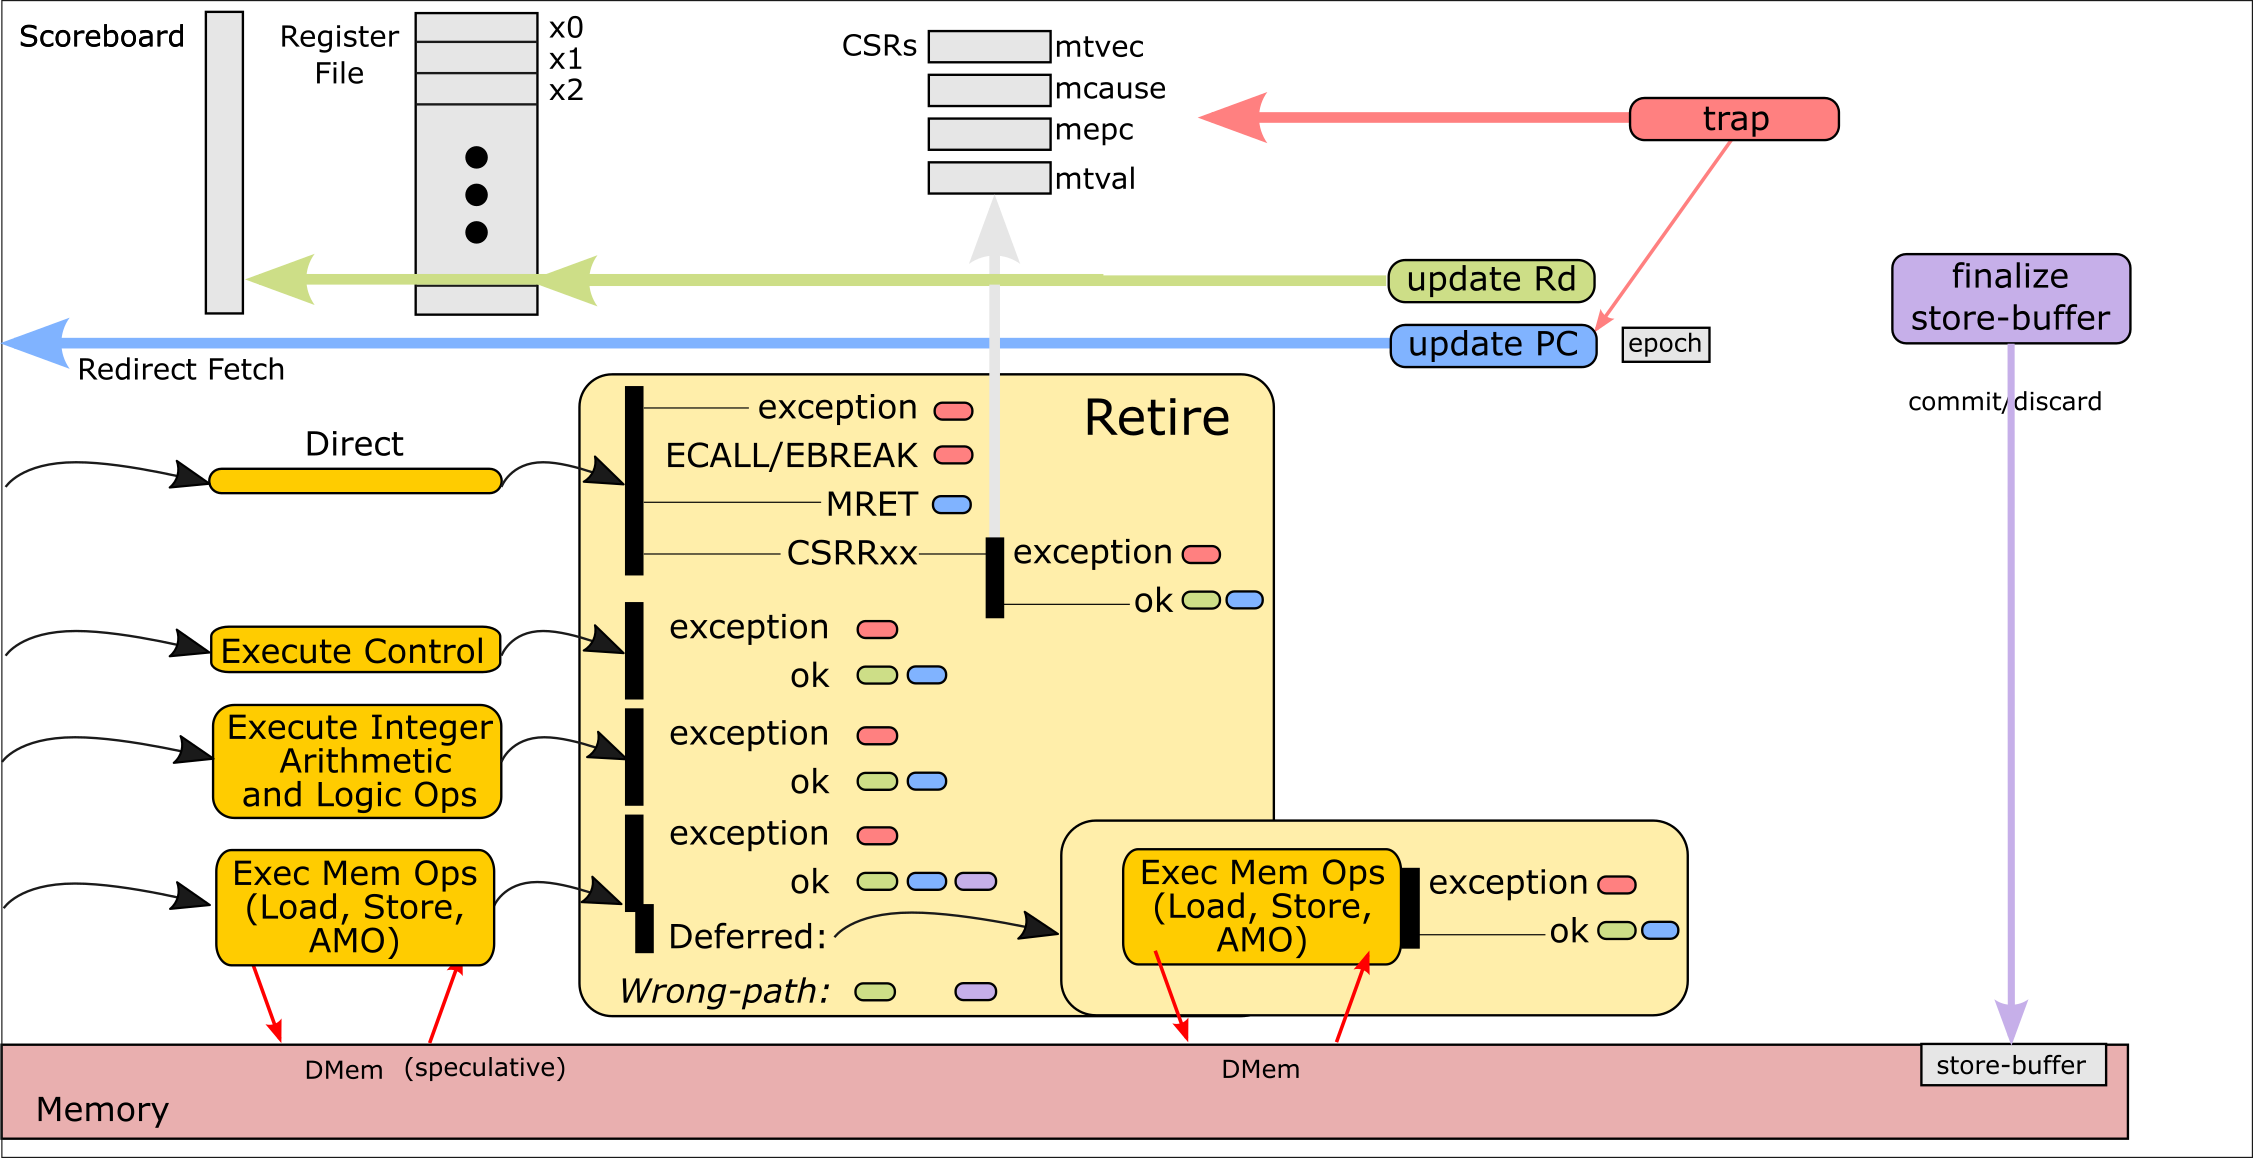
\includegraphics[width=6in,angle=0]{Figures/Fig_Retire_Layers_1_2}}
  \caption{\label{Fig_Fife_Retire_2}
           Actions in the ``Retire'' stage of Fife
	   (same as Fig.~\ref{Fig_Fife_Retire})}
\end{figure}

Here is the interface definition for this module:

{\small
\begin{Verbatim}[frame=single, numbers=left, label=(In file:src\_Fife/S5\_Retire.bsv)]
interface Retire_IFC;
   method Action init (Initial_Params initial_params);

   // Forward in
   interface FIFOF_I #(RR_to_Retire)       fi_RR_to_Retire;
   interface FIFOF_I #(Control_to_Retire)  fi_Control_to_Retire;
   interface FIFOF_I #(EX_to_Retire)       fi_IALU_to_Retire;

   // Speculative DMem response and commit/discard
   interface FIFOF_I #(Mem_Rsp)                fi_DMem_S_rsp;
   interface FIFOF_O #(Retire_to_DMem_Commit)  fo_DMem_S_commit;

   // Non-speculative DMem
   interface FIFOF_O #(Mem_Req)  fo_DMem_req;
   interface FIFOF_I #(Mem_Rsp)  fi_DMem_rsp;

   // Backward out
   interface FIFOF_O #(F_from_Retire)      fo_F_from_Retire;
   interface FIFOF_O #(RW_from_Retire)     fo_RW_from_Retire;
endinterface
\end{Verbatim}
}

The first four \verb|fi_XXX| sub-interfaces correspond to the black
arrows entering the Retire module from the left in the figure.  The
next two \verb|fo_XXX| sub-interfaces correspond to the outgoing red
arrows at the bottom of the module, and the next sub-interface
(\verb|fi_DMem_rsp|) is the incoming red arrow at the bottom of the
module returning a non-speculative memory response.  The last two
sub-interfaces are the black output arrows at the top of the module
carrying redirections to the Fetch stage and Register-Writes to the
\verb|RR_RW| module, respectively.

We define a ``state'' for this module:

{\small
\begin{Verbatim}[frame=single, numbers=left, label=(In file:src\_Fife/S5\_Retire.bsv)]
typedef enum {STATE_PIPE,        // Normal pipeline operation
	      STATE_DMEM_RSP     // Handle Non-speculative DMem response
} Module_State
deriving (Bits, Eq, FShow);
\end{Verbatim}
}

Normally the module is in \verb|STATE_PIPE|, acting as the last stage
of the pipeline.  However, in certain circumstances we switch into
non-pipelined ``FSM'' mode, similar to Drum:

\begin{tightlist}

\item to execute non-speculative DMem ops (MMIO/non-memory-like),

\item to execute traps and interrupts (discussed in a later chapter), and

\item to execute CSRRx insructions  (discussed in a later chapter).

\end{tightlist}

Here we see the code for the \verb|mkRetire| module, the Retire stage
(we have elided the BEHAVIOR section which will be discussed shortly).

{\small
\begin{Verbatim}[frame=single, numbers=left, label=(In file:src\_Fife/S5\_Retire.bsv)]
(* synthesize *)
module mkRetire (Retire_IFC);
   // For managing speculation, redirection traps, etc.
   Reg #(Epoch) rg_epoch  <- mkReg (0);

   // Forward in
   // Depth of f_RR_to_Retire should be > longest EX pipe
   FIFOF #(RR_to_Retire)       f_RR_to_Retire      <- mkSizedFIFOF (8);
   FIFOF #(Control_to_Retire)  f_Control_to_Retire <- mkPipelineFIFOF;
   FIFOF #(EX_to_Retire)       f_IALU_to_Retire    <- mkPipelineFIFOF;
   FIFOF #(Mem_Rsp)            f_DMem_S_rsp        <- mkPipelineFIFOF;

   // Forward out
   FIFOF #(Retire_to_DMem_Commit) f_DMem_S_commit  <- mkBypassFIFOF;

   // Backward out
   FIFOF #(F_from_Retire)   f_F_from_Retire  <- mkBypassFIFOF;
   FIFOF #(RW_from_Retire)  f_RW_from_Retire <- mkBypassFIFOF;

   // Non-speculative DMem reqs and rsps
   FIFOF #(Mem_Req)  f_DMem_req  <- mkBypassFIFOF;
   FIFOF #(Mem_Rsp)  f_DMem_rsp  <- mkPipelineFIFOF;

   Reg #(Module_State) rg_state <- mkReg (STATE_PIPE);

   // ================================================================
   // BEHAVIOR

   ... to be discussed shortly ...

   // ================================================================
   // INTERFACE

   method Action init (Initial_Params initial_params);
      ...
   endmethod

   // Forward in
   interface fi_RR_to_Retire      = to_FIFOF_I (f_RR_to_Retire);
   interface fi_Control_to_Retire = to_FIFOF_I (f_Control_to_Retire);
   interface fi_IALU_to_Retire    = to_FIFOF_I (f_IALU_to_Retire);

   // Speculative DMem
   interface fi_DMem_S_rsp        = to_FIFOF_I (f_DMem_S_rsp);
   interface fo_DMem_S_commit     = to_FIFOF_O (f_DMem_S_commit);

   // Non-speculative DMem
   interface fo_DMem_req       = to_FIFOF_O (f_DMem_req);
   interface fi_DMem_rsp       = to_FIFOF_I (f_DMem_rsp);

   // Backward out
   interface fo_F_from_Retire  = to_FIFOF_O (f_F_from_Retire);
   interface fo_RW_from_Retire = to_FIFOF_O (f_RW_from_Retire);
endmodule
\end{Verbatim}
}

The first section (preceding BEHAVIOR) instantiates register
\verb|rg_epoch| to keep track of the epoch, and then FIFOs for all the
incoming and outgoing channels.  Finally, it instantiates register
\verb|rg_state| to hold the current module state.

The final, INTERFACE, section, as before, has an \verb|init| method,
and then lifts the various FIFO interfaces into sub-interfaces for
this module.

The BEHAVIOR section consists of a collection of rules, each handling
a distinct scenario.  In overview:

\begin{itemize}

  \item Rule \verb|rl_Retire_wrong_path| handles all mis-predicted
        instructions.

  \item Rules \verb|rl_Retire_normal| and \verb|rl_Retire_exc| handle
        instructions with \verb|EXEC_TAG_RETIRE|, {\ie} instructions
        that only have a direct message from the
        Register-Read-and-Dispatch stage, with nothing in any of the
        other execution pipelines.

  \item Rules \verb|rl_Retire_Control_normal| and
        \verb|rl_Retire_Control_exc| handle instructions with
        \verb|EXEC_TAG_CONTROL|, {\ie} BRANCH and JAL/JALR
        instructions that came through the Execute Control pipe.

  \item Rules \verb|rl_Retire_Int_normal| and \verb|rl_Retire_Int_exc|
        handle instructions with \verb|EXEC_TAG_INT|---LUI, AUIPC and
        Integer Arithmetic/Logic instructions that came through the
        Execute Int pipe.

  \item Rules \verb|rl_Retire_DMem_S_normal| and
        \verb|rl_Retire_DMem_S_exc| handle instructions with
        \verb|EXEC_TAG_DMEM|---LOAD and STORE instructions that came
        through the Execute DMem pipe---and were executed
        speculatively (into memory-like addresses).

  \item Rules \verb|rl_Retire_DMem_deferred| and
        \verb|rl_Retire_DMem_rsp| handle instructions with
        \verb|EXEC_TAG_DMEM|---LOAD and STORE instructions that came
        through the Execute DMem pipe---and were deferred (not
        executed) because they were for MMIO/non-memory-like addresses.

\end{itemize}

Each pair of rules \verb|rl_XXX_normal| and \verb|rl_XXX_exc| handle
the two cases where the instruction completes normally {\vs} the
instruction has raised an exception (trap).

% ================================================================

\subsection{Common facilities used by many rules}

\label{Sec_Retire_Common}

The following function captures the actions to be taken when we
discover that the prediction for the successor to this instruction was
wrong.  The boolean \verb|mispredicted| indicates whether the
prediction was correct or not.  If the prediction was correct, no
action is taken.  Otherwise, we increment the epoch, and send a
redirection message to the Fetch stage with the correct PC and the new
epoch.  The disposition of this message was discussed in
Section~\ref{Sec_Fife_Fetch_stage}.

{\small
\begin{Verbatim}[frame=single, numbers=left, label=(In file:src\_Fife/S5\_Retire.bsv)]
   // Redirect Fetch stage on mispredicted PC
   function Action fa_redirect_Fetch (Bool         mispredicted,
				      RR_to_Retire x1,
				      Bit #(XLEN)  next_pc);
      action
	 if (mispredicted) begin
	    let next_epoch = rg_epoch + 1;
	    rg_epoch <= next_epoch;
	    let y = F_from_Retire {inum:       x1.inum,
				   pc:         x1.pc,
				   instr:      x1.instr,
				   next_pc:    next_pc,
				   next_epoch: next_epoch};
	    f_F_from_Retire.enq (y);
	 end
      endaction
   endfunction
\end{Verbatim}
}

The following function captures the actions to be taken for updating
an instruction's destination rd register.  It simply assembles a
\verb|RW_to_Retire| message and sends it to the \verb|RR_RW| module.
The disposition of this message was discussed in
Section~\ref{Sec_RR_RW_module}.

{\small
\begin{Verbatim}[frame=single, numbers=left, label=(In file:src\_Fife/S5\_Retire.bsv)]
   // Update Rd for those instructions that have an Rd 
   function Action fa_update_rd (RR_to_Retire x1, Bool commit, Bit #(XLEN) rd_val);
      action
	 let y = RW_from_Retire {inum:       x1.inum,
				 pc:         x1.pc,
				 instr:      x1.instr,
				 rd:         instr_rd (x1.instr),
				 commit:     commit,
				 data:       rd_val};
	 f_RW_from_Retire.enq (y);
      endaction
   endfunction
\end{Verbatim}
}

The following definitions examine the first element of the
\verb|f_RR_to_Retire| (direct path) queue, which controls how incoming
instructions are merged and disposed of, in the rules that follow.

{\small
\begin{Verbatim}[frame=single, numbers=left, label=(In file:src\_Fife/S5\_Retire.bsv)]
   RR_to_Retire x_rr_to_retire = f_RR_to_Retire.first;

   Bool wrong_path = (x_rr_to_retire.epoch != rg_epoch);
   Bool is_Direct  = (x_rr_to_retire.exec_tag == EXEC_TAG_RETIRE);
   Bool is_Control = (x_rr_to_retire.exec_tag == EXEC_TAG_CONTROL);
   Bool is_Int     = (x_rr_to_retire.exec_tag == EXEC_TAG_IALU);
   Bool is_DMem    = (x_rr_to_retire.exec_tag == EXEC_TAG_DMEM);
\end{Verbatim}
}

The incoming instruction is a wrong-path instruction if its
accompanying epoch does not match our \verb|rg_epoch| register.  The
remaining four definitions summarize the class of the instruction
based on the execution tag; these control which of the following rules
will fire.

% ================================================================

\subsection{Rule to discard wrong-path instructions}

For a wrong-path instruction, we must dequeue it from
\verb|f_RR_to_Retire| and any associated Execute queue (Control, Int
or DMem).  It if is a DMem STORE instruction that was performed
speculatively, we must also send a ``discard'' message to the head of
the store-buffer.  Finally, if the instruction has an rd destination
register, we must send an discard-scoreboard-reservation message to
the RR-RW module using the \verb|fa_update_rd| function described in
the Section~\ref{Sec_Retire_Common}.

{\small
\begin{Verbatim}[frame=single, numbers=left, label=(In file:src\_Fife/S5\_Retire.bsv)]
   rule rl_Retire_wrong_path ((rg_state == STATE_PIPE)
			      && wrong_path);
      f_RR_to_Retire.deq;

      if (is_Control) f_Control_to_Retire.deq;
      if (is_Int)     f_IALU_to_Retire.deq;
      if (is_DMem) begin
	 f_DMem_S_rsp.deq;

	 // Send discard to Store Buffer, if needed
	 Bool commit_store_val = ((! is_LOAD (x_rr_to_retire.instr))
				  && (! is_LR (x_rr_to_retire.instr))
				  && (f_DMem_S_rsp.first.rsp_type == MEM_RSP_OK));
	 if (commit_store_val) begin
	    let y = Retire_to_DMem_Commit{inum:   x_rr_to_retire.inum,
					  commit: False};
	    f_DMem_S_commit.enq (y);
	 end
      end

      // Release rd scoreboard reservation, if has one
      Bool rd_commit = False;
      if (x_rr_to_retire.has_rd) fa_update_rd (x_rr_to_retire, rd_commit, ?);
   endrule
\end{Verbatim}
}

% ================================================================

\subsection{Rules to retire instructions direct from RR-RW}

The following rules handle instructions that are direct from the RR-RW
stage, {\ie} which were \emph{not} also sent through any of the
Execute pipes (Control, Int or DMem).

If it is not an exception, then it must be a CSRRx instruction, which
we have not yet implemented yet (we will do so in
Chapter~\ref{ch_Fife_Exception}).  For now, we treat it as a no-op.  We
dequeue the instruction from \verb|f_RR_to_Retire|.  For CSRRx
instructions, the correct next-PC is the fall-through PC, so we check
this against the predicted PC, and redirect if necessary using
action-function \verb|fa_redirect_fetch()| which was described in
Section~\ref{Sec_Retire_Common}.

{\small
\begin{Verbatim}[frame=single, numbers=left, label=(In file:src\_Fife/S5\_Retire.bsv)]
   rule rl_Retire_normal ((rg_state == STATE_PIPE)
                          && (! wrong_path)
                          && is_Direct
			  && (! x_rr_to_retire.exception));
      f_RR_to_Retire.deq;

      $display ("CSRRx instructions not yet implemented; no-op for now");

      // Redirect Fetch PC if mispredicted
      Bool mispredicted = (x_rr_to_retire.predicted_pc
                           != x_rr_to_retire.fallthru_pc);
      fa_redirect_Fetch (mispredicted, x_rr_to_retire, x_rr_to_retire.fallthru_pc);
   endrule
\end{Verbatim}
}

If the first element of \verb|f_RR_to_Retire| is carrying an
exception, this could be due to a memory-fault during Fetch, or
detection of an illegal instruction during Decode.  In
Chapter~\ref{ch_Fife_Exception} we will describe how to handle
exceptions, but for now we use \verb|$finish()| to abort the
simulation.

{\small
\begin{Verbatim}[frame=single, numbers=left, label=(In file:src\_Fife/S5\_Retire.bsv)]
   rule rl_Retire_exc ((rg_state == STATE_PIPE)
                       && (! wrong_path)
		       && is_Direct
		       && x_rr_to_retire.exception);
      f_RR_to_Retire.deq;

      $display ("Exception-handling not yet implemented");
      $finish (1);
   endrule
\end{Verbatim}
}

% ================================================================

\subsection{Rules to retire instructions from the Execute Control path}

If the instruction is a Control instruction without an exception, we
pop the relevant incoming queues (\verb|f_RR_to_Retire| and
\verb|f_Control_to_Retire|), update the Rd destination register (JAL
and JALR often save a ``return address'' in rd), and redirect the
Fetch stage if mispredicted.

{\small
\begin{Verbatim}[frame=single, numbers=left, label=(In file:src\_Fife/S5\_Retire.bsv)]
   rule rl_Retire_Control_normal ((rg_state == STATE_PIPE)
                                  && (! wrong_path)
				  && is_Control
				  && (! f_Control_to_Retire.first.exception));
      f_RR_to_Retire.deq;
      let x2 <- pop_o (to_FIFOF_O (f_Control_to_Retire));

      // Updata rd if valid
      Bool rd_commit = True;
      if (x2.data_valid) fa_update_rd (x_rr_to_retire, rd_commit, x2.data);

      // Redirect Fetch PC if mispredicted
      Bool mispredicted = (x_rr_to_retire.predicted_pc != x2.next_pc);
      fa_redirect_Fetch (mispredicted,  x_rr_to_retire, x2.next_pc);
   endrule
\end{Verbatim}
}

If the instruction is carrying an exception this is because the
BRANCH, JAL or JALR target was misaligned.  In
Chapter~\ref{ch_Fife_Exception} we will describe how to handle
exceptions, but for now we use \verb|$finish()| to abort the
simulation.

{\small
\begin{Verbatim}[frame=single, numbers=left, label=(In file:src\_Fife/S5\_Retire.bsv)]
   rule rl_Retire_Control_exc ((rg_state == STATE_PIPE)
                               && (! wrong_path)
                               && is_Control
			       && f_Control_to_Retire.first.exception);
      f_RR_to_Retire.deq;
      let x2 <- pop_o (to_FIFOF_O (f_Control_to_Retire));

      $display ("Exception-handling not yet implemented");
      $finish (1);
   endrule
\end{Verbatim}
}

% ================================================================

\subsection{Rules to retire instructions from the Execute Int path}

The two rules to retire instructions from the Execute Int path are
similar to the rules for the Control path in the previous section.

If the instruction is without an exception, we pop the relevant
incoming queues (\verb|f_RR_to_Retire| and \verb|f_IALU_to_Retire|),
update the Rd destination register, and redirect the Fetch stage if
mispredicted.

{\small
\begin{Verbatim}[frame=single, numbers=left, label=(In file:src\_Fife/S5\_Retire.bsv)]
   rule rl_Retire_Int_normal ((rg_state == STATE_PIPE)
			      && (! wrong_path)
			      && is_Int
			      && (! f_IALU_to_Retire.first.exception));
      f_RR_to_Retire.deq;
      EX_to_Retire x2 <- pop_o (to_FIFOF_O (f_IALU_to_Retire));

      // Updata rd if valid
      Bool rd_commit = True;
      if (x2.data_valid) fa_update_rd (x_rr_to_retire, rd_commit, x2.data);

      // Redirect Fetch PC if mispredicted
      Bool mispredicted = (x_rr_to_retire.predicted_pc != x_rr_to_retire.fallthru_pc);
      fa_redirect_Fetch (mispredicted, x_rr_to_retire, x_rr_to_retire.fallthru_pc);
   endrule
\end{Verbatim}
}

If the instruction is carrying an exception: in
Chapter~\ref{ch_Fife_Exception} we will describe how to handle
exceptions, but for now we use \verb|$finish()| to abort the
simulation.

{\small
\begin{Verbatim}[frame=single, numbers=left, label=(In file:src\_Fife/S5\_Retire.bsv)]
   rule rl_Retire_Control_exc ((rg_state == STATE_PIPE)
                               && (! wrong_path)
                               && is_Control
			       && f_Control_to_Retire.first.exception);
      f_RR_to_Retire.deq;
      let x2 <- pop_o (to_FIFOF_O (f_Control_to_Retire));

      $display ("Exception-handling not yet implemented");
      $finish (1);
   endrule
\end{Verbatim}
}

Note, none of the standard RISC-V Integer instructions raise any
exceptions, so we do not expect this rule to ever be
executed. However, if we extend the ISA to new Integer instructions
that could raise an exception, this rule is ready to field those
exceptions.

% ================================================================

\subsection{Rules to retire instructions from the Execute DMem path}

From the Execute DMem path we receive memory responses.  If the
response type is \verb|MEM_RSP_OK| then this instruction was executed
speculatively and successfully; we just have to retire it just like
the Control and Int scenarios above, with the additional need to send
a ``commit'' message to the store-buffer if it wrote to memory.

{\small
\begin{Verbatim}[frame=single, numbers=left, label=(In file:src\_Fife/S5\_Retire.bsv)]
   rule rl_Retire_Dmem_S_normal ((rg_state == STATE_PIPE)
				 && (! wrong_path)
				 && is_DMem
				 && (f_DMem_S_rsp.first.rsp_type == MEM_RSP_OK));
      f_RR_to_Retire.deq;
      let x2 <- pop_o (to_FIFOF_O (f_DMem_S_rsp));

      Bool rd_commit = True;
      if (x_rr_to_retire.has_rd)
	 fa_update_rd (x_rr_to_retire, rd_commit, truncate (x2.data));

      // Send commit to Store Buffer if it wrote to memory
      Bool wrote_mem = ((! is_LOAD (x_rr_to_retire.instr))
		        && (! is_LR (x_rr_to_retire.instr)));
      if (wrote_mem) begin
	 let y = Retire_to_DMem_Commit{inum:   x_rr_to_retire.inum,
				       commit: True};
	 f_DMem_S_commit.enq (y);
      end

      // Redirect Fetch PC if mispredicted
      Bool mispredicted = (x_rr_to_retire.predicted_pc != x_rr_to_retire.fallthru_pc);
      fa_redirect_Fetch (mispredicted, x_rr_to_retire, x_rr_to_retire.fallthru_pc);
   endrule
\end{Verbatim}
}

If the DMem response indicates that it attempted a speculative access
and encountered an exception, the memory response type will be
\verb|MEM_RSP_ERR| or \verb|MEM_RSP_MISALIGNED|.  We compute the
appropriate RISC-V exception \verb|cause| code.  In
Chapter~\ref{ch_Fife_Exception} we will describe how to handle
exceptions, but for now we use \verb|$finish()| to abort the
simulation.

{\small
\begin{Verbatim}[frame=single, numbers=left, label=(In file:src\_Fife/S5\_Retire.bsv)]
   Bool dmem_S_rsp_exception = ((f_DMem_S_rsp.first.rsp_type    == MEM_RSP_ERR)
				|| (f_DMem_S_rsp.first.rsp_type == MEM_RSP_MISALIGNED));

   rule rl_Retire_Dmem_S_exc ((rg_state == STATE_PIPE)
			      && (! wrong_path)
			      && is_DMem
			      && dmem_S_rsp_exception);
      f_RR_to_Retire.deq;
      let x2 <- pop_o (to_FIFOF_O (f_DMem_S_rsp));

      Bit #(XLEN)  cause = ?;
      if (x2.rsp_type == MEM_RSP_MISALIGNED)
	 cause = (is_LOAD (x_rr_to_retire.instr)
		  ? cause_LOAD_ADDRESS_MISALIGNED
		  : cause_STORE_AMO_ADDRESS_MISALIGNED);
      else
	 cause = (is_LOAD (x_rr_to_retire.instr)
		  ? cause_LOAD_ACCESS_FAULT
		  : cause_STORE_AMO_ACCESS_FAULT);

      $display ("Exception-handling not yet implemented");
      $finish (1);
   endrule
\end{Verbatim}
}

If the DMem response indicates that it deferred the request because
the address was to an MMIO/non-memory-like address, the memory
response type will be \verb|MEM_RSP_ERR| or \verb|MEM_REQ_DEFERRED|.
In this case, we now construct the memory response and send it to
memory.  Finally we change the module state to \verb|STATE_DMEM_RSP|
indicating that we will now await the memory response.  Note, this all
previous rules will no longer fire because they all have
``\verb|(rg_state == STATE_PIPE)|'' in their rule conditions, which is
now false.

{\small
\begin{Verbatim}[frame=single, numbers=left, label=(In file:src\_Fife/S5\_Retire.bsv)]
   rule rl_Retire_DMem_deferred ((rg_state == STATE_PIPE)
                                 && (! wrong_path)
				 && is_DMem
				 && (f_DMem_S_rsp.first.rsp_type == MEM_REQ_DEFERRED));
      let x2 <- pop_o (to_FIFOF_O (f_DMem_S_rsp));
      let mem_req = Mem_Req{inum:     x2.inum,
			    pc:       x2.pc,
			    instr:    x2.instr,
			    req_type: x2.req_type,
			    size:     x2.size,
			    addr:     x2.addr,
			    data:     x2.data};
      f_DMem_req.enq (mem_req);
      rg_state <= STATE_DMEM_RSP;
   endrule
\end{Verbatim}
}

The final rule, handles the corresponding responses from memory.  We
pop the direct-path information (\verb|f_RR_to_Retire|) and the
memory-response (\verb|f_DMem_Rsp|).

If the response returned an exception, we compute the RISC-V exception
\verb|cause|.  In Chapter~\ref{ch_Fife_Exception} we will describe how
to handle exceptions, but for now we use \verb|$finish()| to abort the
simulation.

Next we check for \verb|MEM_REQ_DEFERRED| responses.  This is a
redundant check in that it should be impossible---the non-speculative
DMem port should never defer any requests---and is just a bit of
defensive programming in case of a bug in the memory system.  We abort
the simulation with \verb|$finish()|.

On successful responses (\verb|MEM_RSP_OK|) we perform the usual
writeback-register and possible redirection on misprediction.

Finally, we set \verb|rg_state| to \verb|STATE_PIPE|, which once again
enables all the pipeline rules.

{\small
\begin{Verbatim}[frame=single, numbers=left, label=(In file:src\_Fife/S5\_Retire.bsv)]
   rule rl_Retire_DMem_rsp (rg_state == STATE_DMEM_RSP);
      f_RR_to_Retire.deq;
      let mem_rsp <- pop_o (to_FIFOF_O (f_DMem_rsp));

      Bool exception = ((mem_rsp.rsp_type == MEM_RSP_ERR)
			|| (mem_rsp.rsp_type == MEM_RSP_MISALIGNED));
      Bit #(XLEN)  cause = ?;
      if (exception) begin
	 if (mem_rsp.rsp_type == MEM_RSP_MISALIGNED)
	    cause = (is_LOAD (x_rr_to_retire.instr)
		     ? cause_LOAD_ADDRESS_MISALIGNED
		     : cause_STORE_AMO_ADDRESS_MISALIGNED);
	 else
	    cause = (is_LOAD (x_rr_to_retire.instr)
		     ? cause_LOAD_ACCESS_FAULT
		     : cause_STORE_AMO_ACCESS_FAULT);
	 $finish (1);
      end
      else if (mem_rsp.rsp_type == MEM_REQ_DEFERRED) begin
         $display ("IMPOSSIBLE: Unexpected MEM_REQ_DEFERRED; FINISH.");
	 $finish (1);
      end
      else begin
      	 // mem_rsp.rsp_type will be MEM_REQ_OK here

	 // Writeback register
	 Bool rd_commit = True;
	 if (x_rr_to_retire.has_rd)
	    fa_update_rd (x_rr_to_retire, rd_commit, truncate (mem_rsp.data));

	 // Redirect Fetch to correct mispredicted PC
	 fa_redirect_Fetch ((x_rr_to_retire.predicted_pc != x_rr_to_retire.fallthru_pc),
			    x_rr_to_retire,
			    x_rr_to_retire.fallthru_pc);
      end
      // Go back to pipeline behavior
      rg_state <= STATE_PIPE;
   endrule
\end{Verbatim}
}

Note that in this module, when we have a DMem response with
response-type \verb|MEM_REQ_DEFERRED| we effectively switch from
pipeline processing to Drum-like FSM processing (one FSM state issues
a DMem request and another FSM state fields the response and processes
it).  This is a standard trick: for an instruction that cannot for
some reason be pipelined, we execute it completely in the Retire
module in Drum-like FSM mode.  In fact, we shall use exactly this
trick to implement CSRRxx instructions (in
Chapter~\ref{ch_Fife_CSRRxx}, because CSRRx instructions are tricky to
execute in the main pipeline.

% ****************************************************************
